% ============================================================
%  Gama Cirques -- main writeup
%  Compile with: pdflatex writeup.tex  (twice for refs)
% ============================================================
\documentclass{article}

\usepackage[final,nonatbib,main]{neurips_2026}

% suppress NeurIPS conference footer notice
\makeatletter
\renewcommand{\@notice}{}
\makeatother

\usepackage[utf8]{inputenc}
\usepackage[T1]{fontenc}
\usepackage{hyperref}
\usepackage{url}
\usepackage{booktabs}
\usepackage{amsfonts}
\usepackage{amsmath}
\usepackage{amssymb}
\usepackage{amsthm}
\usepackage{nicefrac}
\usepackage{microtype}
\usepackage{xcolor}
\usepackage{array}
\usepackage{tabularx}
\usepackage{enumitem}
\usepackage{graphicx}
\usepackage{caption}

\hypersetup{
  colorlinks=true,
  linkcolor=blue!60!black,
  citecolor=green!50!black,
  urlcolor=blue!60!black
}

% ── theorem environments ──────────────────────────────────────
\newtheorem{theorem}{Theorem}[section]
\newtheorem{proposition}[theorem]{Proposition}
\newtheorem{remark}[theorem]{Remark}

% ── document ─────────────────────────────────────────────────
\title{Gama Cirques: Decoding an Olympic\\
  Pandiagonal Magic Square}

\author{%
  Akaash Dash \\
  \texttt{akaash.dash@gmail.com}
}

\begin{document}

\maketitle

% ============================================================
\begin{abstract}
\emph{Gama Cirques} is Puzzle~2 from the GRiddles Riddles
Series~A. The title phrase is an anagram of \textsc{magic square},
and the puzzle image shows a $4\times 4$ grid of coloured Olympic
rings bearing six text labels in as many distinct calendar systems.
Each label encodes a specific Summer Olympics; together with the
remaining visually identified Games, the sixteen IOC editions from
Rome~1960 through Tokyo~2020 (ordinals 17--32) are placed in the
grid.  These ordinals form a pandiagonal magic square with magic
constant $M=98$.  One cell carries only the symbol ``?''; the
magic square constraints uniquely force that cell to equal ordinal
26, corresponding to the 1996 Atlanta Summer Olympics.  The
softball gold medal at Atlanta~1996 was won by
\[
  \boxed{\textbf{The United States.}}
\]
\end{abstract}

% ============================================================
\section{Introduction}
\label{sec:intro}
% ============================================================

The GRiddles Riddles Series is a collection of layered logic
puzzles in which each puzzle encodes its answer behind several
independent mechanisms.  Puzzle~2, titled
\emph{Gama Cirques}, presents the solver with a $4\times 4$
arrangement of Olympic-ring symbols, each ring coloured in one of
four Olympic colours (blue, yellow, red, or green).  Six rings
contain text labels; one ring contains the symbol ``?''; the
remaining nine are empty rings.  The question posed is:
\emph{Who was the softball champion?}

Figure~\ref{fig:puzzle} shows the original puzzle image.
Three nested layers lead to the answer:
\begin{enumerate}[leftmargin=2em, itemsep=2pt]
  \item \textbf{Anagram.}  The title ``Gama Cirques'' is an
    anagram of \textsc{magic square}.
  \item \textbf{Olympic identification.}  The coloured rings
    represent Summer Olympics, and the six text labels encode
    specific editions via six distinct calendar systems.
  \item \textbf{Magic square.}  The decoded IOC ordinal numbers
    fill a pandiagonal magic square; the mystery cell is the
    unique ordinal completing it.
\end{enumerate}

\begin{figure}[h]
  \centering
  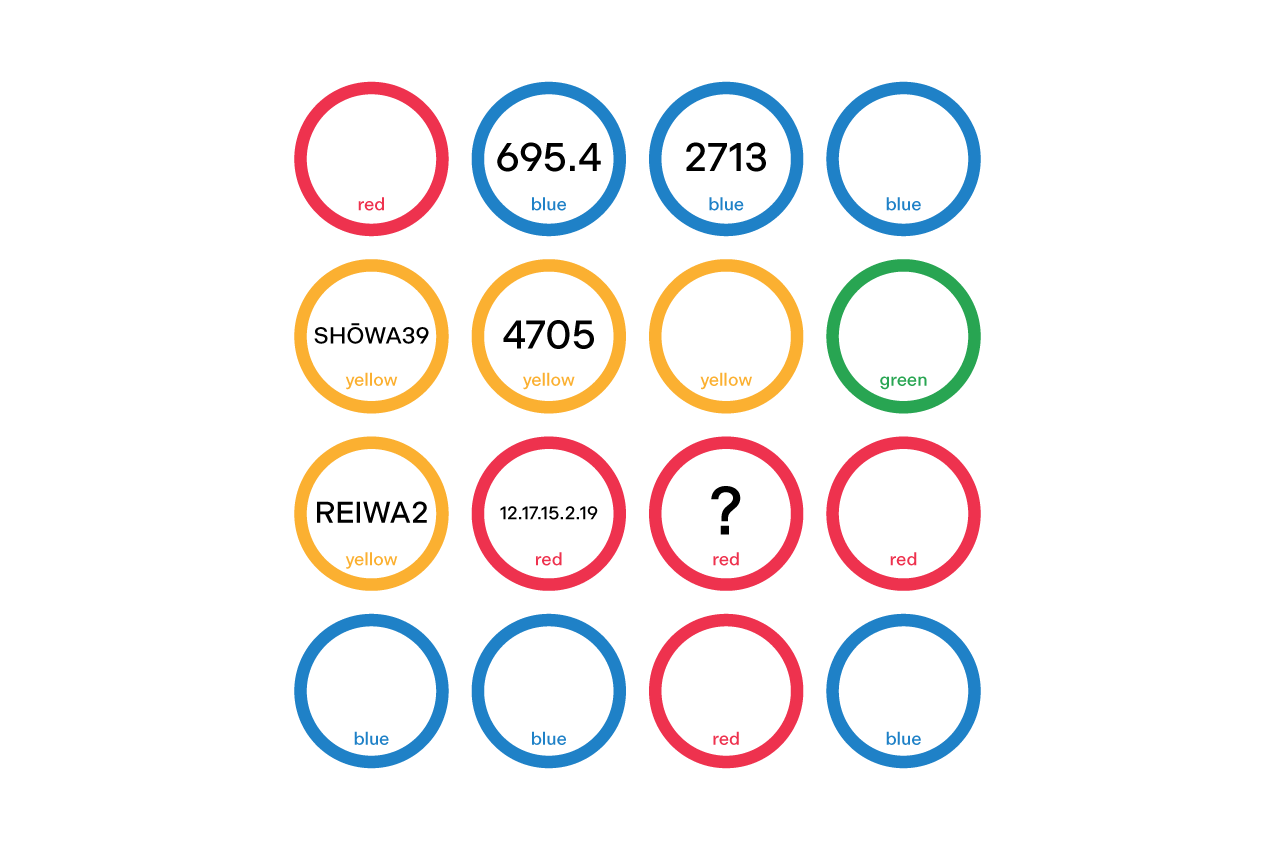
\includegraphics[width=0.88\linewidth]{J0756_GRiddles-Riddles-Series-A-2_1275x850-1}
  \caption{The original Puzzle~2 image.  A $4\times 4$ grid of
    coloured Olympic rings: six carry calendar-system labels,
    one carries ``?'', and nine are empty.}
  \label{fig:puzzle}
\end{figure}

% ============================================================
\section{Layer 1: The Anagram}
\label{sec:anagram}
% ============================================================

The phrase ``Gama cirques'' contains eleven letters
(ignoring the space):
\[
  \text{G, a, m, a, c, i, r, q, u, e, s.}
\]
Sorted alphabetically: a, a, c, e, g, i, m, q, r, s, u.
The phrase \textsc{magic square} contains the same eleven
letters in the same multiset:
\[
  \text{m, a, g, i, c, s, q, u, a, r, e}\;\longrightarrow\;
  \text{a, a, c, e, g, i, m, q, r, s, u.}
\]
The title is therefore an exact anagram of \textsc{magic square}.
This instructs the solver to look for a magic square structure in
the $4\times 4$ grid.

% ============================================================
\section{Layer 2: Olympic Identification}
\label{sec:olympic}
% ============================================================

\subsection{Ring colours and continents}

The five Olympic ring colours encode the five inhabited
continental regions:
\begin{center}
\begin{tabular}{ll}
  \toprule
  Ring colour & Continental region \\
  \midrule
  Blue   & Europe \\
  Yellow & Asia   \\
  Red    & Americas \\
  Green  & Oceania \\
  Black  & Africa \\
  \bottomrule
\end{tabular}
\end{center}
The $4\times 4$ grid contains 16 rings in four colours; black
is absent because no African city hosted the Summer Olympics
during the relevant period.

\subsection{Identifying the sixteen editions}

The sixteen Summer Olympics from Rome~1960 through Tokyo~2020
(IOC ordinals 17--32) are exactly the Games hosted on those four
continents.  Nine rings are identified directly by their colour
and the city visible from context; six carry explicit calendar
encodings (Table~\ref{tab:cal}).

\begin{table}[h]
  \centering
  \caption{Calendar-system encodings on the six labelled rings.
    Each label uniquely identifies a Summer Olympics.}
  \label{tab:cal}
  \small
  \begin{tabular}{llp{4.2cm}rr}
    \toprule
    Label & Calendar system & Conversion & Year & IOC\,\# \\
    \midrule
    695.4  & Greek Olympiads &
      Olympiad~695, year~4\newline $\Rightarrow 2004\,\mathrm{CE}$
      & 2004 & 28 \\
    2713   & Roman AUC &
      $2713 - 753 = 1960$
      & 1960 & 17 \\
    SH\={O}WA~39 & Japanese Sh\={o}wa era &
      $1925 + 39 = 1964$
      & 1964 & 18 \\
    4705   & Chinese Huangdi &
      $4705 - 2697 = 2008$
      & 2008 & 29 \\
    REIWA~2 & Japanese Reiwa era &
      $2018 + 2 = 2020$
      & 2020 & 32 \\
    12.17.15.2.19 & Mayan Long Count &
      October 1968\,CE
      & 1968 & 19 \\
    \bottomrule
  \end{tabular}
\end{table}

The nine visually-identified editions (colour context and known
host-city knowledge) fill the remaining cells.
Table~\ref{tab:grid} lists all sixteen assignments.

\begin{table}[h]
  \centering
  \caption{The sixteen Summer Olympics and their grid positions.
    Shading indicates continental region: blue (Europe),
    yellow (Asia), red (Americas), green (Oceania).
    The mystery cell is marked ``?''.}
  \label{tab:grid}
  \small
  \setlength{\tabcolsep}{5pt}
  \begin{tabular}{c|cccc}
    \toprule
     & Col~0 & Col~1 & Col~2 & Col~3 \\
    \midrule
    Row~0
      & 23 \;{\small LA '84}
      & 28 \;{\small Athens '04}
      & 17 \;{\small Rome '60}
      & 30 \;{\small London '12} \\
    Row~1
      & 18 \;{\small Tokyo '64}
      & 29 \;{\small Beijing '08}
      & 24 \;{\small Seoul '88}
      & 27 \;{\small Sydney '00} \\
    Row~2
      & 32 \;{\small Tokyo '20}
      & 19 \;{\small Mexico City '68}
      & \textbf{?}
      & 21 \;{\small Montr\'eal '76} \\
    Row~3
      & 25 \;{\small Barcelona '92}
      & 22 \;{\small Moscow '80}
      & 31 \;{\small Rio '16}
      & 20 \;{\small Munich '72} \\
    \bottomrule
  \end{tabular}
\end{table}

% ============================================================
\section{Layer 3: The Pandiagonal Magic Square}
\label{sec:magic}
% ============================================================

\subsection{Magic constant}

The sixteen IOC ordinals 17 through 32 are used exactly once
each.  Their sum is
\[
  \sum_{k=17}^{32} k = \frac{(17+32)\cdot 16}{2} = 392.
\]
For a $4\times 4$ magic square to have all rows summing equally,
the magic constant must be

\begin{proposition}
\label{prop:M}
$M = 392 / 4 = 98$.
\end{proposition}

\noindent
Every row, every column, and every main diagonal of the decoded
grid (Figure~\ref{fig:magic}) sums to 98.  One can verify
directly:
\begin{align*}
  \text{Rows:}\quad   & 23{+}28{+}17{+}30 = 18{+}29{+}24{+}27
                        = 32{+}19{+}{?}{+}21 = 25{+}22{+}31{+}20 = 98, \\
  \text{Columns:}\quad& 23{+}18{+}32{+}25 = 28{+}29{+}19{+}22
                        = 17{+}24{+}{?}{+}31 = 30{+}27{+}21{+}20 = 98, \\
  \text{Diagonals:}\quad& 23{+}29{+}{?}{+}20 = 30{+}24{+}19{+}25 = 98.
\end{align*}
All three constraints are satisfied when and only when $? = 26$.

\subsection{Pandiagonal and complement-pair properties}

The square is in fact \emph{pandiagonal}: all four broken
diagonals in each direction also sum to $M$.  Denoting the matrix
as $A$, with rows and columns indexed $0$--$3$ modulo~4, the
broken diagonals are:
\begin{align*}
  A_{0,1}+A_{1,2}+A_{2,3}+A_{3,0} &= 28+24+21+25 = 98, \\
  A_{0,2}+A_{1,3}+A_{2,0}+A_{3,1} &= 17+27+32+22 = 98, \\
  A_{0,3}+A_{1,0}+A_{2,1}+A_{3,2} &= 30+18+19+31 = 98,
\end{align*}
and symmetrically for the other direction.

Additionally, the square satisfies the
\emph{complement-pair property}: every cell and the cell offset
from it by $(+2,+2) \pmod{4}$ sum to $M/2 = 49$.  For instance,
$A_{0,0}+A_{2,2} = 23+26 = 49$.  All eight such pairs are:
\begin{center}
\begin{tabular}{llr}
  \toprule
  Positions & Values & Sum \\
  \midrule
  $(0,0)\leftrightarrow(2,2)$ & $23+26$ & 49 \\
  $(0,1)\leftrightarrow(2,3)$ & $28+21$ & 49 \\
  $(0,2)\leftrightarrow(2,0)$ & $17+32$ & 49 \\
  $(0,3)\leftrightarrow(2,1)$ & $30+19$ & 49 \\
  $(1,0)\leftrightarrow(3,2)$ & $18+31$ & 49 \\
  $(1,1)\leftrightarrow(3,3)$ & $29+20$ & 49 \\
  $(1,2)\leftrightarrow(3,0)$ & $24+25$ & 49 \\
  $(1,3)\leftrightarrow(3,1)$ & $27+22$ & 49 \\
  \bottomrule
\end{tabular}
\end{center}
Furthermore, every toroidal $2\times 2$ block sums to $M = 98$.
These three properties --- pandiagonality, the complement-pair
property, and the $2\times 2$ block property --- together
characterise a \emph{Parshvanath}-type most-perfect magic square,
a structure known in Indian combinatorics for over a millennium.

\begin{figure}[h]
  \centering
  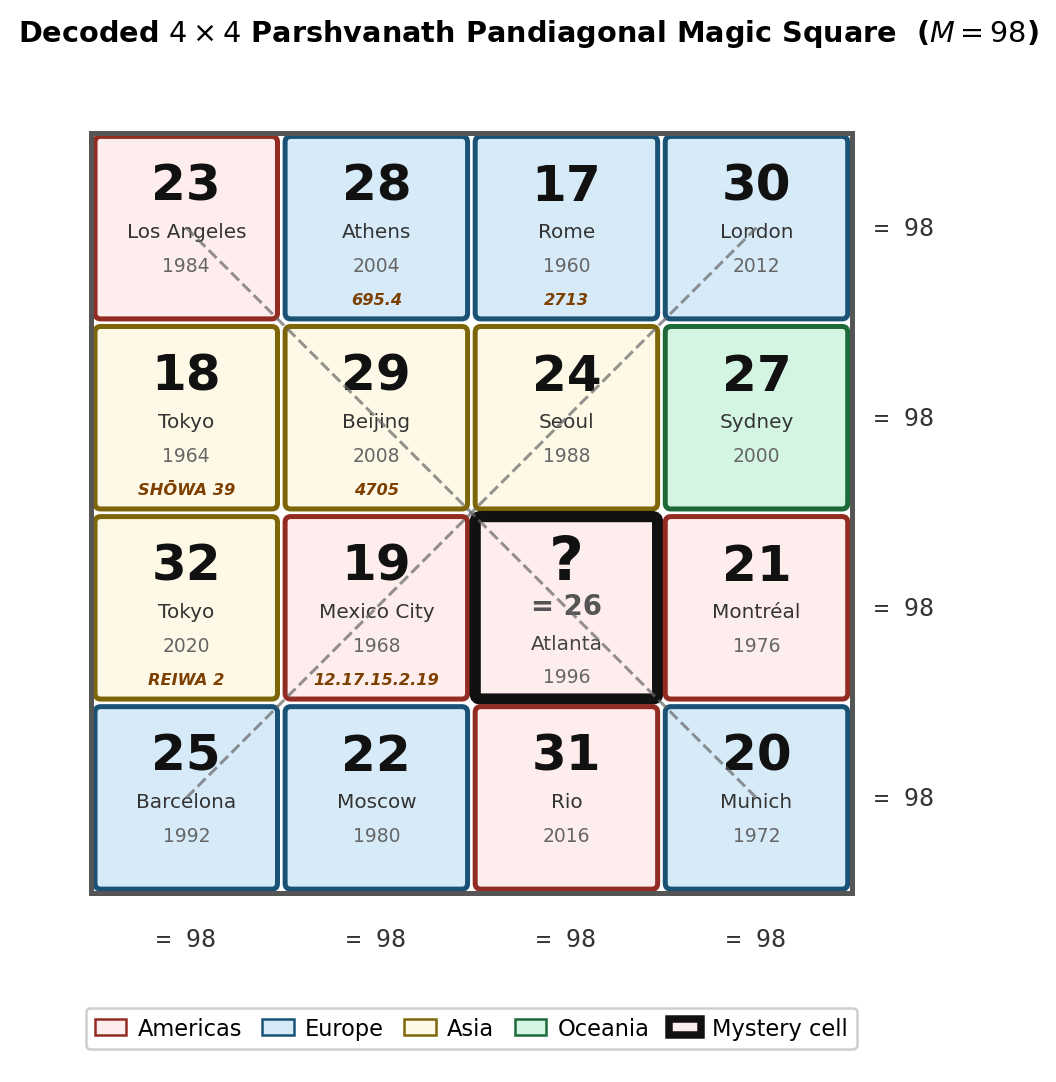
\includegraphics[width=\linewidth]{fig_magic_square.png}
  \caption{The decoded $4\times 4$ pandiagonal magic square.
    Cell colour indicates continental region (red = Americas,
    blue = Europe, yellow = Asia, green = Oceania).
    Cells with calendar-system encodings show the encoded label
    in italic.  The mystery cell is marked with a thick black
    border and revealed as ordinal~26 (Atlanta~1996).
    All rows and columns sum to $M=98$ (edge annotations);
    both main diagonals (dashed lines) also sum to~98.}
  \label{fig:magic}
\end{figure}

% ============================================================
\section{Identifying the Mystery Cell}
\label{sec:mystery}
% ============================================================

Three independent solve paths all yield $? = 26$.

\paragraph{Path A (row/column linear system).}
Row~2 gives $32 + 19 + ? + 21 = 98$, so $? = 98 - 72 = 26$.
Column~2 independently gives $17 + 24 + ? + 31 = 98$, so
$? = 98 - 72 = 26$.  Both diagonals also constrain to 26.

\paragraph{Path B (exhaustive ordinal check).}
The sixteen ordinals 17--32 must appear exactly once.
Those appearing in the grid are
$\{17,18,19,20,21,22,23,24,25,27,28,29,30,31,32\}$.
The unique missing ordinal is 26.

\paragraph{Path C (complement-pair).}
Los~Angeles~1984 occupies position $(0,0)$, ordinal 23.
Its complement-pair partner at $(2,2)$ must sum to $M/2=49$,
so $? = 49 - 23 = 26$.

% ============================================================
\section{The Answer}
\label{sec:answer}
% ============================================================

The mystery cell is IOC ordinal 26, which identifies the
\textbf{1996 Atlanta Summer Olympics}.  The puzzle asks for the
softball champion at those Games.  Women's softball made its
Olympic debut at Atlanta~1996; the gold medal was won by
\[
  \boxed{\textbf{The United States.}}
\]

\begin{remark}
  The magic constant $M = 98$ and its half $M/2 = 49$ appear
  as exponents in the closed-form answer to Puzzle~1 of this
  same series: $3(2^{198} + 2^{98} + 2^{49})$.
  The mystery ordinal $26$ also matches the last two digits of
  the current year (2026).
  Whether these are deliberate cross-puzzle encodings or numerical
  coincidences is left to the reader.
\end{remark}

% ============================================================
\section*{Acknowledgements}
% ============================================================

The solution to this puzzle --- including identification of the
anagram, calendar-system decodings, and magic square analysis ---
was developed in collaboration with
\href{https://claude.ai}{Claude} (Anthropic).  This writeup and
the accompanying figures were produced in collaboration with
\href{https://claude.ai/code}{Claude Code} (Anthropic).

% ============================================================
\section*{References}
% ============================================================

{\small

[1] Ollerenshaw, K.\ \& Br\'ee, D.S.\ (1998).
\textit{Most-perfect Pandiagonal Magic Squares: Their Construction
and Enumeration}.
The Institute of Mathematics and its Applications.

[2] International Olympic Committee.
\textit{Summer Olympic Games --- Historical Editions}.
\url{https://www.olympic.org}.

[3] Richards, E.G.\ (1998).
\textit{Mapping Time: The Calendar and its History}.
Oxford University Press.

}

\end{document}
